
\documentclass[xcolor=pdftex,dvipsnames,table,mathserif,aspectratio=169]{beamer}
\usetheme{default}
\usetheme{metropolis}
\usepackage{minted}
\usepackage{mathtools}
\setbeamersize{text margin left=.3in,text margin right=.3in} 

\DeclarePairedDelimiter\abs{\lvert}{\rvert}%
\DeclarePairedDelimiter\norm{\lVert}{\rVert}%

\usepackage[english]{babel}
\usepackage{pgf,pgfarrows,pgfnodes,pgfautomata,pgfheaps}
\usepackage{amsmath,amssymb,setspace,centernot}
\usepackage[latin1]{inputenc}
\usepackage{pgf,tikz}
\usepackage[T1]{fontenc}
\usepackage{relsize}
\usepackage{pdfpages}
\usepackage[absolute,overlay]{textpos} 


\newenvironment{reference}[2]{% 
  \begin{textblock*}{\textwidth}(#1,#2) 
      \footnotesize\it\bgroup\color{red!50!black}}{\egroup\end{textblock*}} 

\DeclareMathSizes{10}{10}{6}{6} 

\begin{document}
\title{Part 9: Marginal Treatment Effects}
\author{Chris Conlon}
\institute{Applied Econometrics}
\date{\today}

\maketitle
\section{Marginal Treatment Effects}


\begin{frame}{Motivation}
We started with by talking about two approaches to program evaluation for $\Delta_i = Y_i(1) - Y_i(0)$.
\begin{itemize}
\item In the \alert{structural approach} the goal was to recover the full distribution $f(\Delta_i)$, and with that recover whichever objects we wanted
\item The other approach focused on characterizing particular moments of the distribution
\begin{align*}
ATT(x) &= E[ \Delta_i | X_i=x, T_{i}=1]\\
ATU(x) &= E[ \Delta_i |  X_i=x,  T_{i}=0]\\
LATE(x) &= E[ \Delta_i |  X_i=x,  T_{i}(z_i=1) > T_{i}(z_i = 0)]
\end{align*}

\item But how exactly are these approaches linked?
\end{itemize}
The answer is through a \alert{nonparametric function} known as the \alert{marginal treatment effect} (MTE).
\end{frame}

\begin{frame}{One quantity to rule them all: MTE}
\begin{itemize}
\item Consider a treatment effect $\Delta_i = Y_{i}(1) - Y_{i}(0)$.
\item Think about a single-index such that $T_i = 1(v_i \leq Z_i' \gamma)$.
\item Think about the person for whom $v_i = Z_i'\gamma$\\
 (indifferent between treatment and non-treatment).
\begin{eqnarray*}
\Delta^{MTE}(x, v_i) = E[\Delta_i | X_i=x, v_i = Z_i'\gamma] 
\end{eqnarray*}
\item Now instead of being \alert{a number} like LATE, the MTE: $\Delta^{MTE}(x, v)$ is a \alert{function} of $v$
\item It is the average impact of receiving a treatment for everyone with the same $Z_i' \gamma$.
\end{itemize}
\end{frame}

\begin{frame}{One quantity to rule them all: MTE}
But what is $Z_i' \gamma$?
\begin{itemize}
\item For any \alert{single index model} we can rewrite 
\begin{eqnarray*}
T_i = \mathbf{1}(v_i \leq Z_i' \gamma) = \mathbf{1}(u_{is} \leq F(Z_i' \gamma)) \mbox{ for }  u_{is} \in [0,1]
\end{eqnarray*}
\item $F$ is just the cdf of $v_i$: (could be logit or probit, or anything else).
\item Use the CDF to write things as a uniform distribution.
\item Now we can write \alert{propensity score} $P(Z_i) = Pr(T_i=1|Z_i )= F(Z_i '\gamma)$.
\end{itemize}
\end{frame}

\begin{frame}{Alternative Definitions}
\begin{itemize}
\item Heckman (1997) also shows the relationship to LATE:
\begin{align*}
\Delta^{MTE}(x, z)= \lim_{z' \rightarrow z} \text{Wald}(z,z',x)
\end{align*}
\item A function where we evaluate the limit of LATE at each value of $z$
\item The alternative way to define the MTE is as \alert{Local IV}:
\begin{eqnarray*}
\Delta^{LIV}(x, p) = \frac{\partial E[Y_i | X_i=x, P(Z_i) =p] }{\partial p}
\end{eqnarray*}
\item How does the outcome $Y_i$ change as we push one more person into treatment (via the \alert{Propensity Score})
\end{itemize}
\end{frame}




\begin{frame}
\frametitle{MTE: Derivation}
Now we can write,
\begin{eqnarray*}
Y(0) &=& \gamma_0' X + U_0\\
Y(1) &=& \gamma_1' X + U_1
\end{eqnarray*}
$P(T=1 | Z) = P(Z)$ works as our instrument with two assumptions:
\begin{enumerate}
\item $(U_0, U_1, u_s) \perp P(Z) | X$. (Exogeneity)
\item Conditional on $X$ there is enough variation in $Z$ for $P(Z)$ to take on all values $\in(0,1)$.
\begin{itemize}
\item This is much stronger than typical \alert{relevance} condition. Much more like the \alert{special regressor} method we will discus later.
\end{itemize}
\end{enumerate}
\end{frame}

\begin{frame}
\frametitle{MTE: Derivation}
\footnotesize
Now we can write,
\begin{eqnarray*}
Y &=& \gamma_0' X + T(\gamma_1 - \gamma_0)' X + U_0 + T(U_1 - U_0)\\
E[Y| X,P(Z)=p] &=& \gamma_0' X + p(\gamma_1 - \gamma_0)'X + E[T(U_1 - U_0)|X,P(Z)=p]
\end{eqnarray*}
Observe $T=1$ over the interval $u_s = [0,p]$ and zero for higher values of $u_s$. Let $U_1-U_0 \equiv \eta$.
\begin{eqnarray*}
E[T(U_1 - U_0) | P(Z) =p,X] &=& \int_{-\infty}^{\infty} \int_{0}^{p} (U_1 - U_0) f((U_1-U_0) | U_s = u_s) d u_s d(U_1 -U_0)\\
E[T(\eta) | P(Z) =p,X] &=& \int_{-\infty}^{\infty} \int_{0}^{p} \eta f(\eta | U_s = u_s)  d\, \eta d\, u_s\\
\end{eqnarray*}
\end{frame}


\begin{frame}
\frametitle{MTE: Derivation}
Recall:
\begin{align*}
E[Y| X,P(Z)=p] &= \gamma_0' X + p(\gamma_1 - \gamma_0)'X + E[T(U_1 - U_0)|X,P(Z)=p]\\
\end{align*}
And the derivative:
\begin{align*}
\Delta^{MTE}(p) = \frac{\partial E[Y | X, P(Z)=p]}{\partial p} &= (\gamma_1 - \gamma_0)'X + \int_{-\infty}^{\infty} \eta f(\eta | U_s =p) d\, \eta\\
&= \underbrace{(\gamma_1 - \gamma_0)'X}_{\alert{ATE(X)}}+ E[\eta | u_s =p]
\end{align*}
What is $E[\eta | u_s =p]$? The expected unobserved gain from treatment of those people who are on the treatment/no-treatment margin $P(Z)=p$.
\end{frame}

\begin{frame}
\footnotesize
\frametitle{Everything is an MTE}
Calculate the outcome given $(X,Z)$ (actually $X$ and $P(Z)=p$).
\begin{align*}
\Delta^{ATE}(x, T=1)&=E\left(\Delta^{MTE} | X=x \right)\\
\Delta^{T T}(x, P(z), T=1)&=E\left(\Delta^{MTE} | X=x, u_{s} \leq P(z)\right)\\
\Delta^{L A T E}\left(x, P(z), P\left(z^{\prime}\right)\right)&=E\left(\Delta^{MTE} | X=x, P\left(z^{\prime}\right) \leq u_s \leq P(z)\right)
\end{align*}
ATE : This one is obvious. We treat everyone!
\begin{eqnarray*}
\int_{-\infty}^{\infty} \Delta^{MTE}(p) = (\gamma_1 - \gamma_0)'X + \underbrace{\int_{-\infty}^{\infty} E(\eta | u_s) d\, u_s}_{0}
\end{eqnarray*}
ATT: Treat only those with a large enough propensity score $P(z)>p$:
\begin{eqnarray*}
TT(x)=\int_{-\infty}^{\infty} \Delta^{MTE}(p,x) \frac{Pr(P(Z | X) > p)}{E[P(Z | X)]} d\,p
\end{eqnarray*}
\end{frame}

\begin{frame}{Everything is an MTE}
LATE: Integrate over the compliers:
\begin{eqnarray*}
LATE(x,z,z')= \frac{1}{P(z) - P(z')} \int_{P(z')}^{P(z)} \Delta^{MTE}(p,x) 
\end{eqnarray*}
OLS and IV are hard:
\begin{align*}
w^{I V}\left(u_{s}\right)=\left[E\left(P(Z) | P(Z)>u_{s}\right)-E(P(Z))\right] \frac{E(P(Z))}{\operatorname{Var}(P(Z))}\\
w^{O L S}\left(u_{s}\right)=1+\frac{E\left(U_{1} | U_{S}=u_{s}\right) h_{1}-E\left(U_{0} | U_{S}=u_{s}\right) h_{0}}{\Delta^{M T E}\left(u_{s}\right)}\\
h_{1}=\frac{E\left(P(Z) | P(Z)>u_{s}\right)}{ E(P(Z))}, \quad h_{0}=\frac{E\left(P(Z) | P(Z)<u_{s}\right)}{E(P(Z))}
\end{align*}
\end{frame}

\begin{frame}
\frametitle{MTE: Parametric Example}
\begin{center}
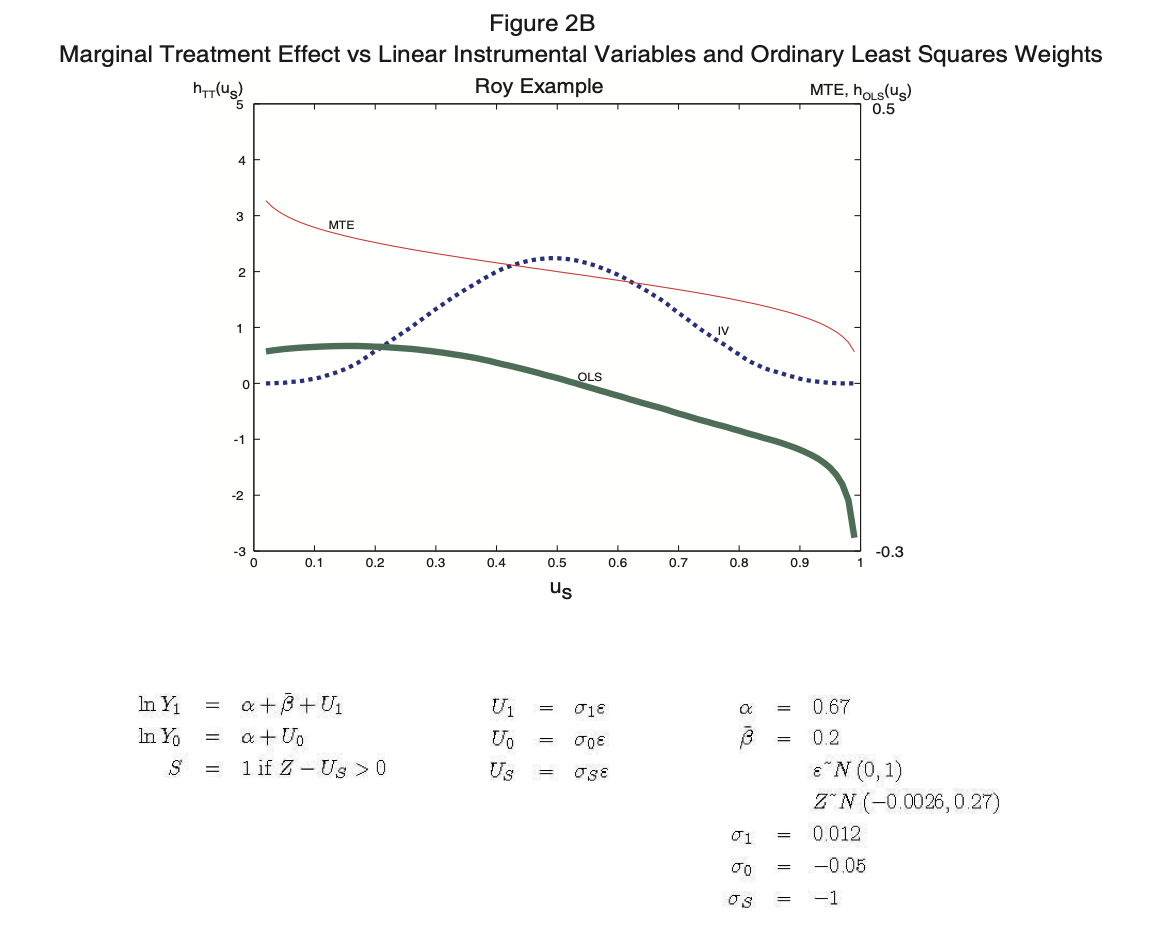
\includegraphics[width=4in]{./resources/mte_plot1.png}
\end{center}
\end{frame}


\begin{frame}
\frametitle{MTE: Parametric Example}
\begin{center}
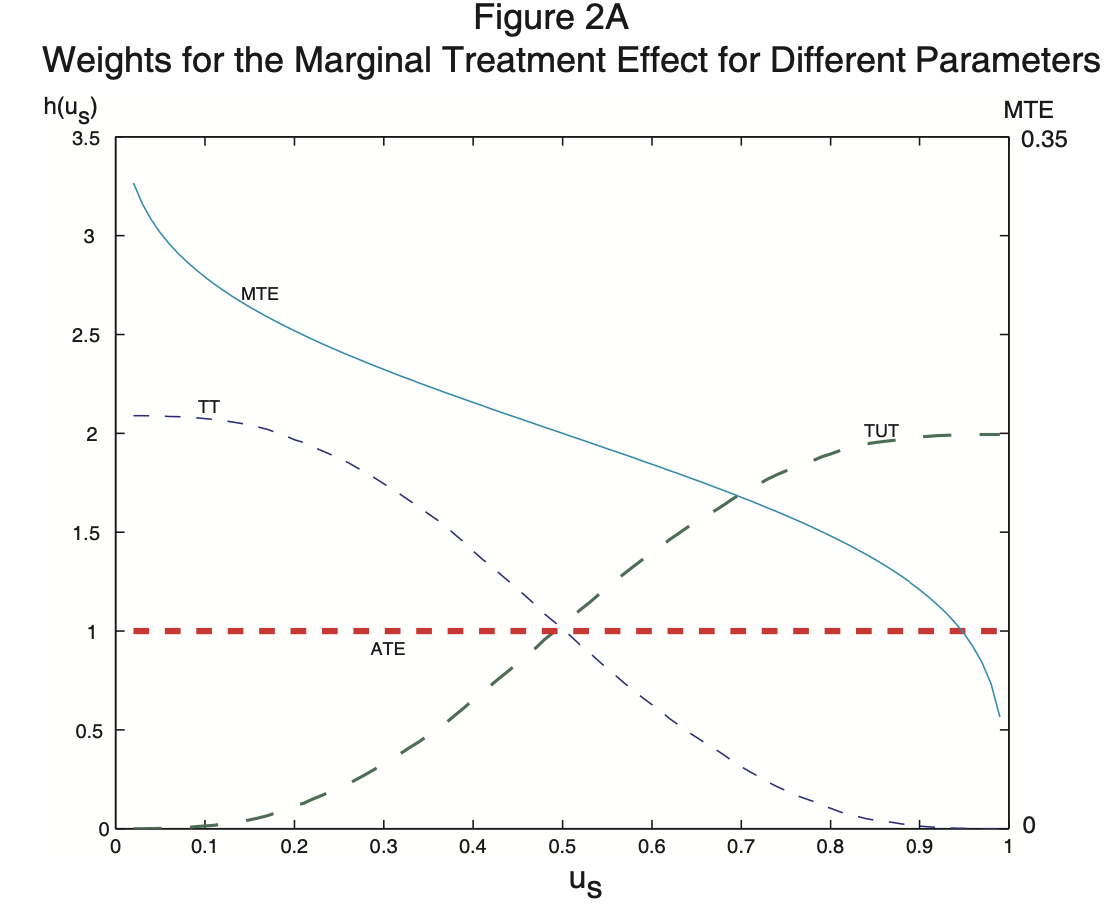
\includegraphics[width=3.5in]{./resources/mte_plot2.png}
\end{center}
\end{frame}



\begin{frame}
\frametitle{How to Estimate an MTE}
Easy?
\begin{enumerate}
\item Estimate $P(Z) = Pr(T=1 | Z)$ nonparametrically (include exogenous part of $X$ in $Z$).
\item Nonparametric regression of $Y$ on $X$ and $P(Z)$ (polynomials?)
\item Differentiate w.r.t. $P(Z)$
\item plot it for all values of $P(Z)=p$.
\end{enumerate}
So long as $P(Z)$ covers $(0,1)$ then we can trace out the full distribution of $\Delta^{MTE}(p)$.
\end{frame}



\begin{frame}
\frametitle{Carneiro, Heckman and Vytlacil (AER 2010)}
\begin{itemize}
\item Estimate returns to college (including heterogeneity of returns).
\item NLSY 1979
\item $Y = \log(wage)$
\item Covariates $X$: Experience (years), Ability (AFQT Score), Mother's Education, Cohort Dummies, State Unemployment, MSA level average wage.
\item Instruments $Z$: College in MSA at age 14, average earnings in MSA at 17 (opportunity cost), avg unemployment rate in state.
\end{itemize}
\end{frame}


\begin{frame}
\frametitle{Carneiro, Heckman and Vytlacil}
\begin{center}
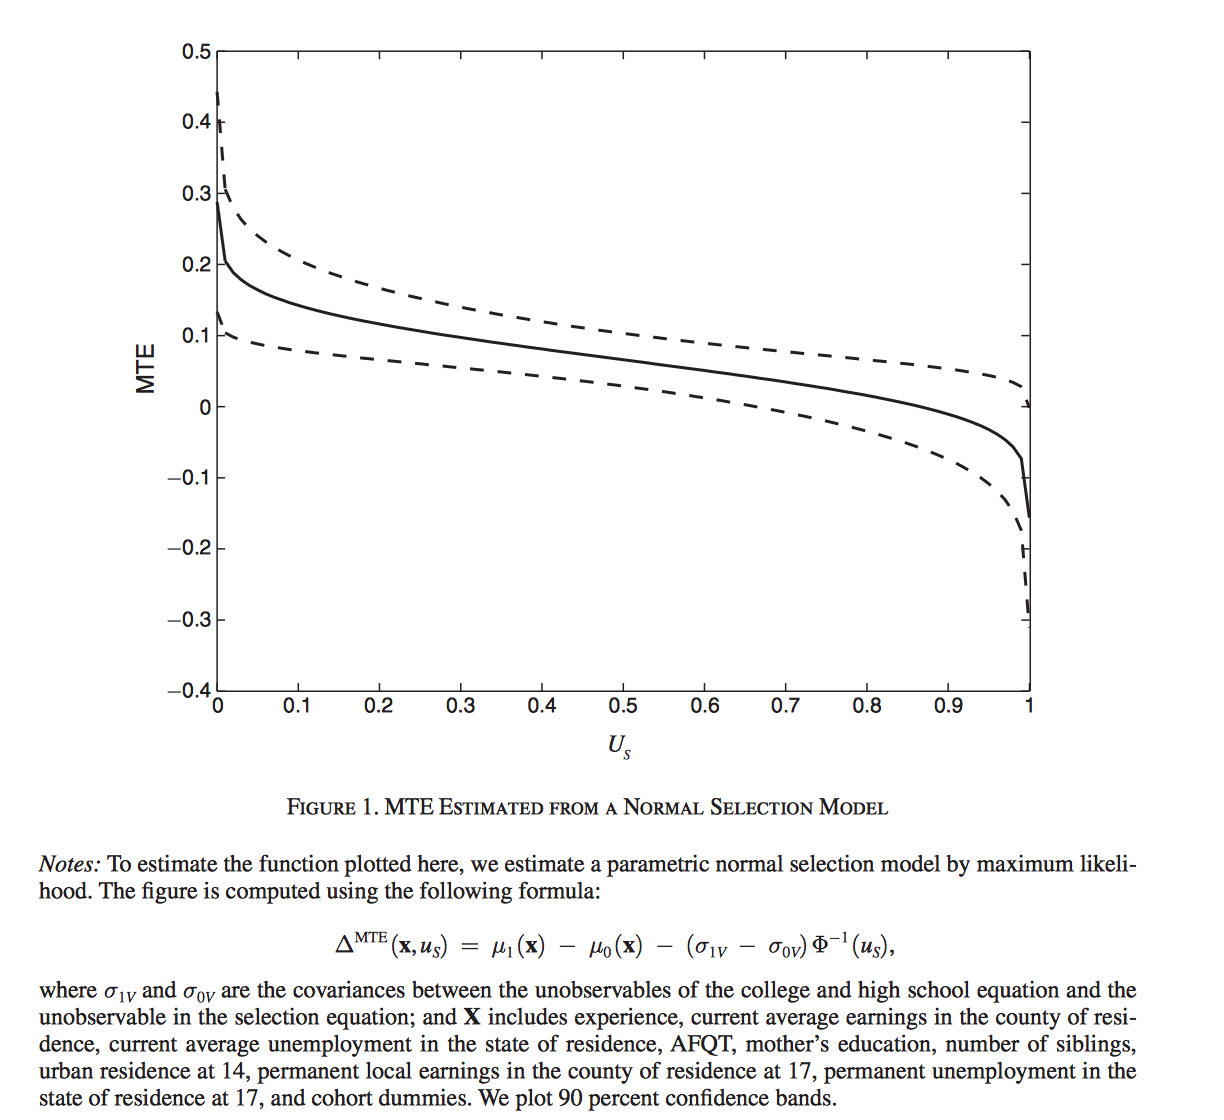
\includegraphics[width=3.5in]{./resources/chv_fig1}
\end{center}
\end{frame}

\begin{frame}
\frametitle{Carneiro, Heckman and Vytlacil}
\begin{center}
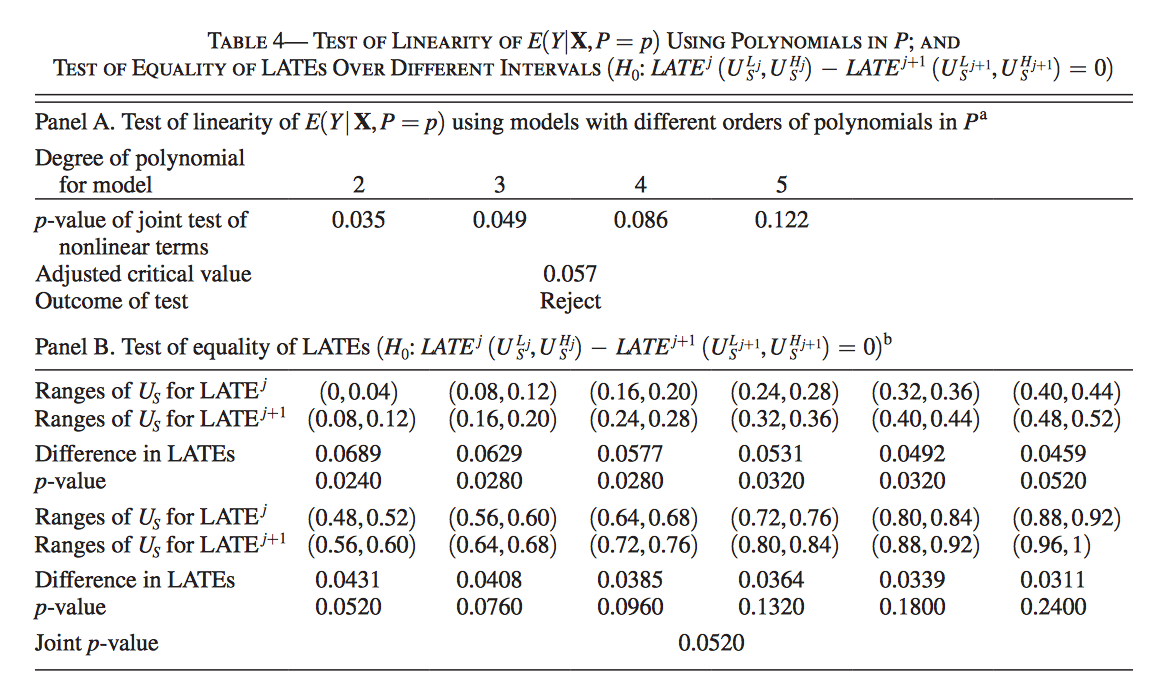
\includegraphics[width=4in]{./resources/chv_tab4}
\end{center}
\end{frame}

\begin{frame}
\frametitle{Carneiro, Heckman and Vytlacil}
\begin{center}
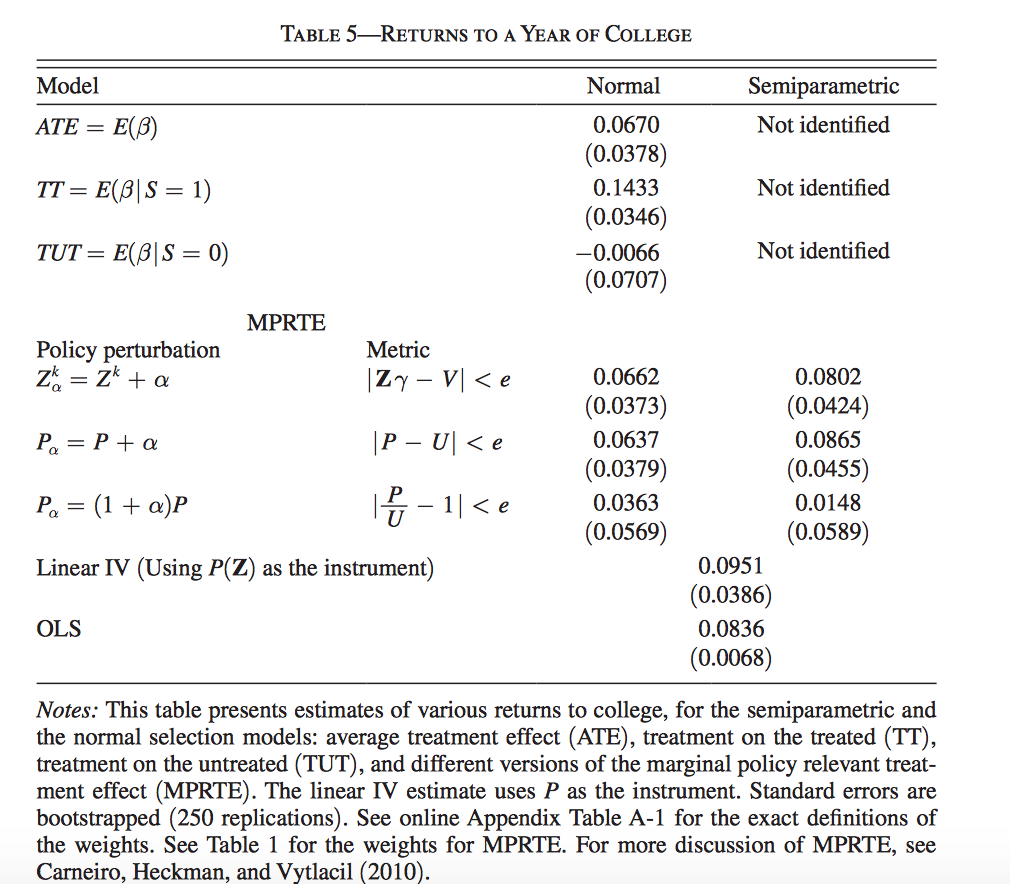
\includegraphics[width=3.5in]{./resources/chv_tab5}
\end{center}
\end{frame}

\begin{frame}
\frametitle{Carneiro, Heckman and Vytlacil}
\begin{center}
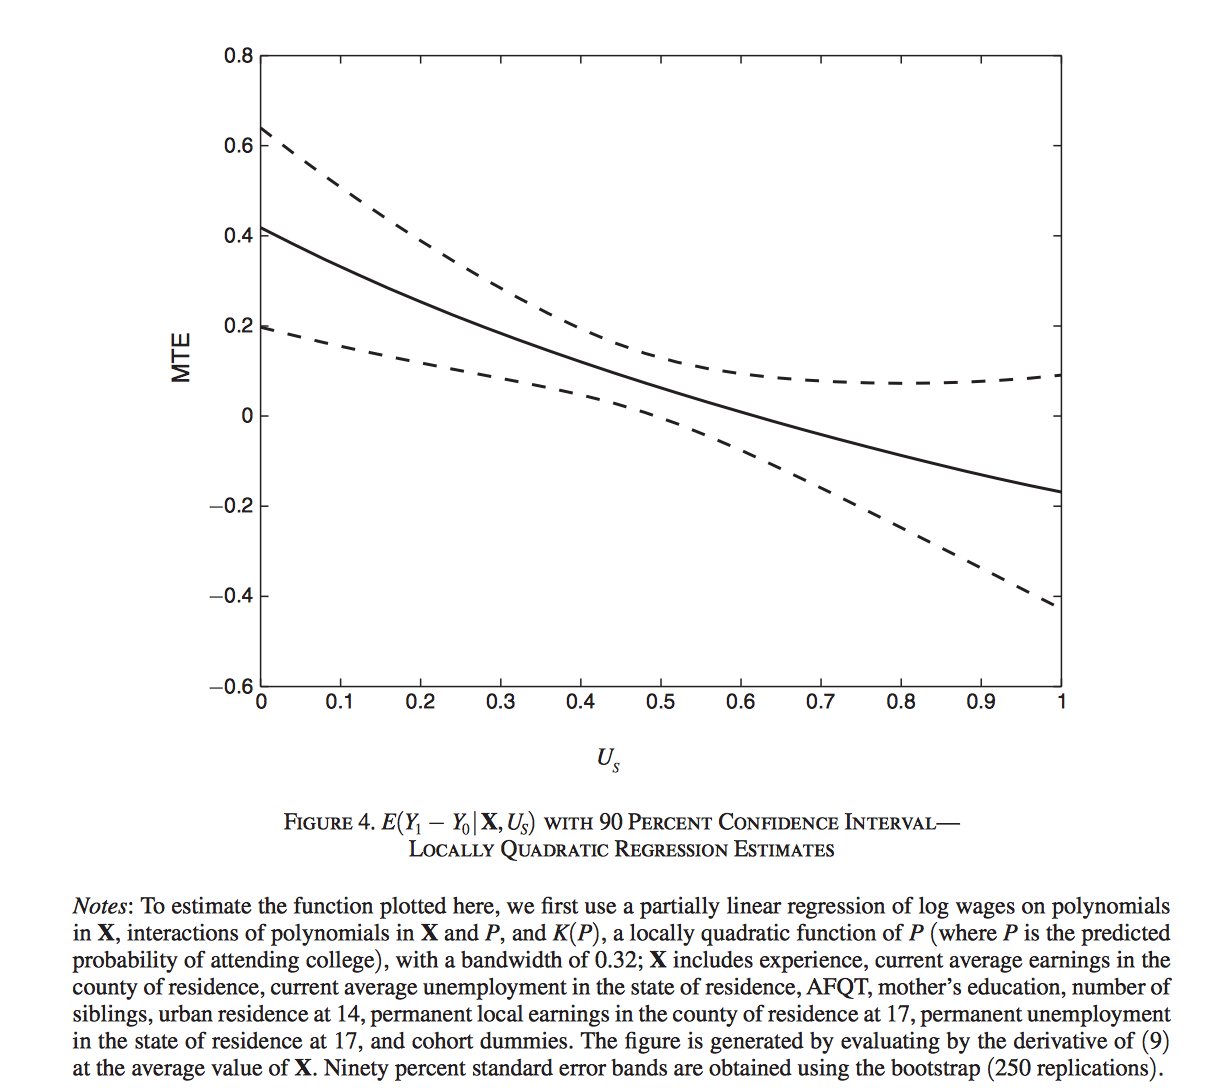
\includegraphics[width=3.5in]{./resources/chv_fig4}
\end{center}
\end{frame}

\begin{frame}
\frametitle{Carneiro, Heckman and Vytlacil}
\begin{center}
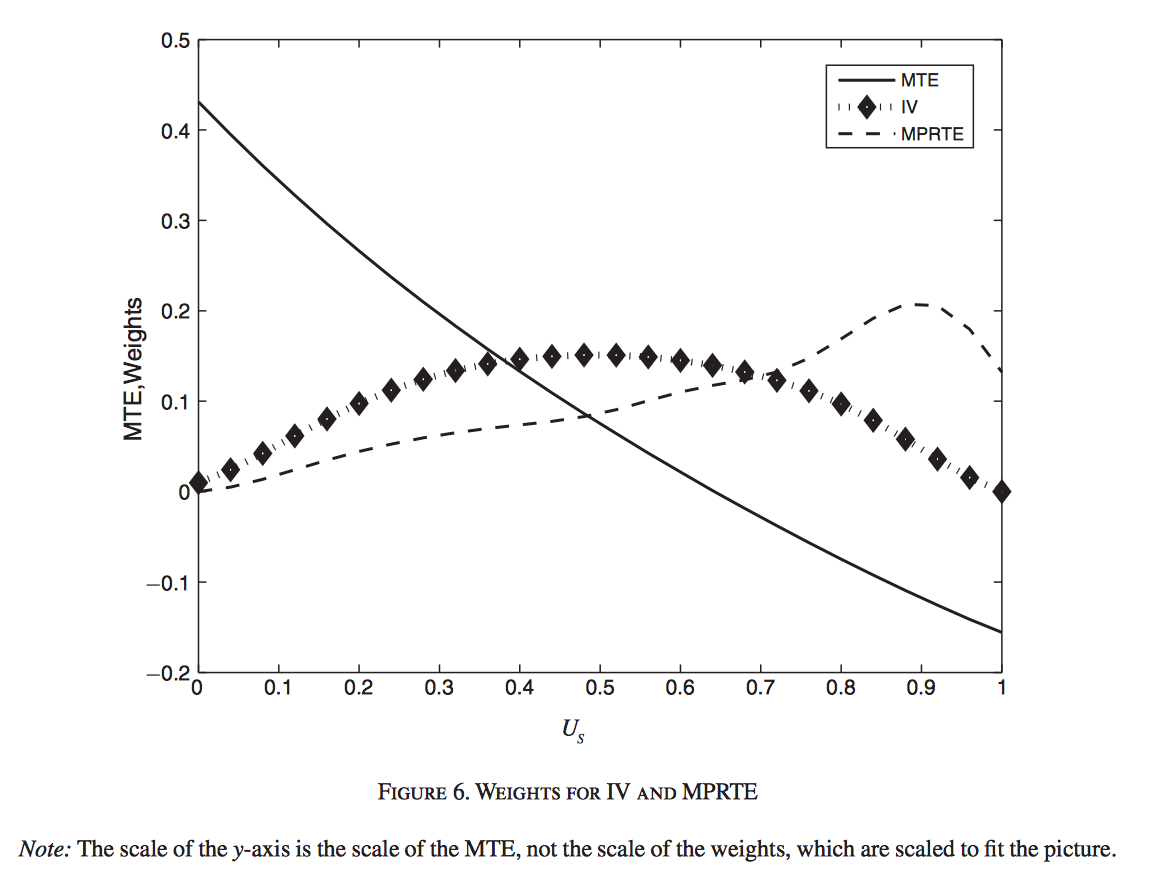
\includegraphics[width=4in]{./resources/chv_fig6}
\end{center}
\end{frame}

%
%\begin{frame}
%\frametitle{Diversion Example}
%I have done some work trying to bring these methods into merger analysis.
%\begin{itemize}
%\item Key quantity: \alert{Diversion Ratio} as I raise my price, how much do people switch to a particular competitor's product
%\begin{eqnarray*}
%D_{jk}(p_j,p_{-j}) = \left| \frac{\partial q_k}{\partial p_j}(p_j,p_{-j}) /  \frac{\partial q_j}{\partial p_j}(p_j,p_{-j}) \right|
%\end{eqnarray*}
%\item We hold $p_{-j}$ fixed and trace out $D_{jk}(p_j)$.
%\item The \alert{treatment} is leaving good $j$.
%\item The $Y_i$ is increased sales of good $k$.
%\item The $Z_i$ is the price of good $j$.
%\item The key is that all changes in sales of $k$ come through people leaving good $j$ (no direct effects).
%\end{itemize}
%\end{frame}
%
%\begin{frame}
%\frametitle{Diversion for Prius (FAKE!)}
%\begin{center}
%%\includegraphics[width=4in]{./resources/sillydiversion.pdf}
%\end{center}
%\end{frame}
%
%\begin{frame}
%\frametitle{Diversion Example}
%\begin{eqnarray*}
%\label{weighteddiversion}
%\widehat{D_{jk}^{LATE} }&=& \frac{1}{\Delta q_j} \int_{p_j^{0}}^{p_j^{0}+\Delta p_j} \underbrace{\frac{\partial q_k(p_j,p^{0}_{-j})}{\partial q_j}}_{\equiv D_{jk}(p_j,p^{0}_{-j})} \left| \frac{\partial q_j(p_j,p^{0}_{-j})}{\partial p_j} \right|\, dp_j
%\end{eqnarray*}
%\begin{itemize}
%\item $D_{jk}(p_j,p^{0}_{-j})$ is the MTE.
%\item Weights $w(p_j) = \frac{1}{\Delta q_j} \frac{\partial q_j(p_j,p^{0}_{-j})}{\partial p_j}$ correspond to the lost sales of $j$ at a particular $p_j$ as a fraction of all lost sales.
%\item When is $LATE \approx ATE$? 
%\begin{itemize}
%\item Demand for Prius is steep: everyone leaves right away
%\item $D_{j,k}(p_j)$ is relatively flat.
%\item We might want to think about raising the price to choke price (or eliminating the product from the consumers choice set) same as treating everyone!
%\end{itemize}
%\end{itemize}
%\end{frame}

\end{document}